\documentclass{article}
\usepackage[T1]{fontenc}
\usepackage{lmodern}
\usepackage{graphicx}
\usepackage{amsmath,amssymb}
\usepackage[a4paper,margin=2cm]{geometry}
\usepackage[absolute,overlay]{textpos}
\setlength{\TPHorizModule}{1mm}
\setlength{\TPVertModule}{1mm}
\usepackage[indonesian]{babel}
\usepackage{hyperref}
\setlength{\emergencystretch}{2em}
% unit: Halaman 10

\begin{document}

% === Halaman 10 (python/native) ===

• Analogi pertukaran kunci Diffie-Hellman adalah seperti 

pertukaran cat antara dua orang (Alice dan Bob).

• Mula-mula Alice dan Bob menyepakati cat bersama  yang 

warnanya tidak perlu rahasia (misalnya cat berwarna kuning)

• Masing-masing Alice dan Bob memiliki cat warna lain yang  

rahasia (dalam hal ini merah dan biru cyan)

• Alice dan Bob mencampurkan cat kuning dengan cat rahasia 

mereka masing-masing. Misalkan hasil pencampurannya 

adalah cat oranye dan cat biru terang

• Kemudian Alice dan Bob saling mempertukarkan cat hasil 

pencampuran tersebut (dikirim melalui transportasi umum).

• Selanjutnya, Alice dan Bob mencampurkan lagi  cat rahasianya 

masing-masing dengan cat hasil pertukaran tersebut.

• Sekarang Alice dan Bob memilik cat berwarna sama yang 

rahasia.

Sumber gambar: Wikipedia

Rinaldi M/II4020 Kriptografi

10

% deskripsi: gambar native xref 61
\noindent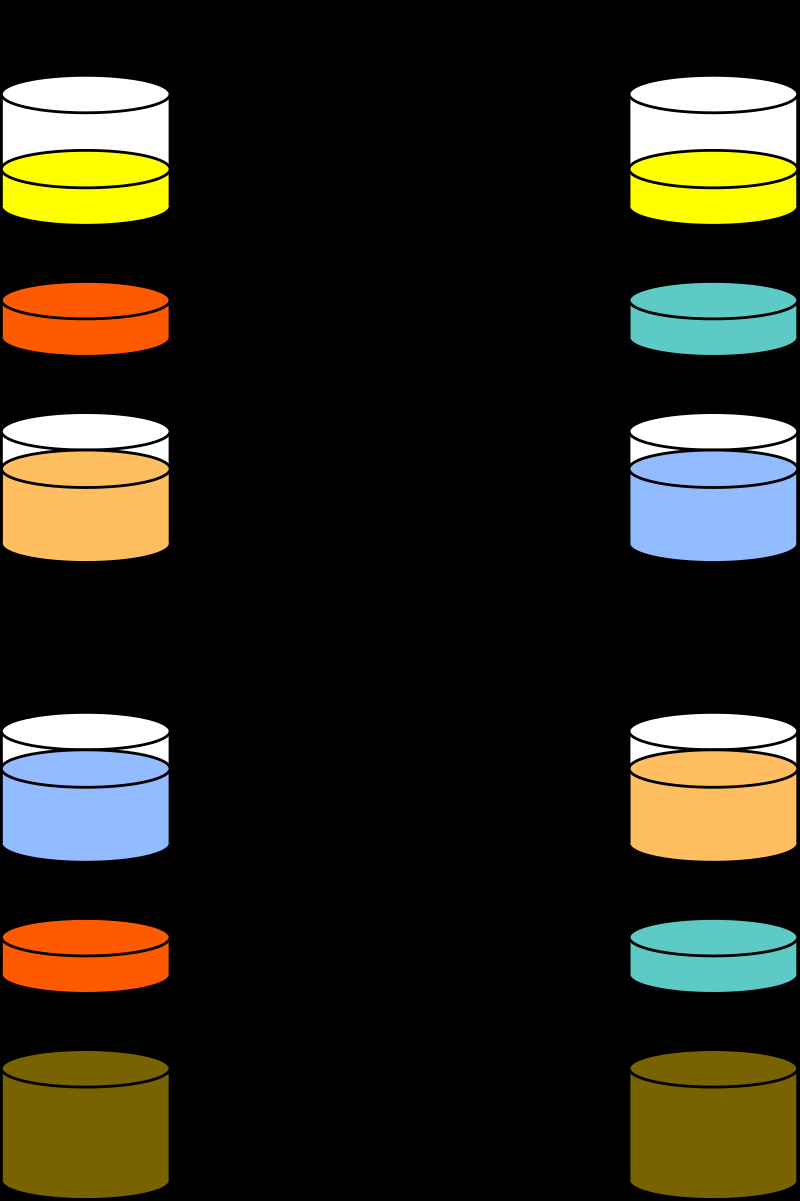
\includegraphics[width=0.85\textwidth]{../../images/python/page_010_img_01.png}

\end{document}
